\documentclass[a4paper,11pt]{article}
\usepackage[T1]{fontenc}
\usepackage[utf8]{inputenc}
\usepackage[english]{babel}
\usepackage{amsmath,amssymb,mathtools}
\usepackage[margin=2.2cm]{geometry}
\usepackage{xcolor,tikz}
\usepackage[most]{tcolorbox}
\setlength{\parindent}{0pt}
\setlength{\parskip}{4pt}
\allowdisplaybreaks
\providecommand{\explainmode}{0}
\newif\ifexplain
\ifnum\explainmode=1 \explaintrue\fi
\newcommand{\aufgabe}[1]{\section*{Exercise #1}}
\newcommand{\angabe}[1]{\textit{#1}\par\smallskip}
\newcommand{\teil}[1]{\subsection*{#1}}
\newcommand{\why}[1]{\text{\small\color{black!65}#1}}
\newtcolorbox{erklbox}{colback=blue!4,colframe=blue!40,breakable,boxrule=0.5pt,title={Erklärung}}
\newcommand{\explain}[1]{\ifexplain\begin{erklbox}#1\end{erklbox}\fi}
\newcommand{\explainfig}[1]{\ifexplain\begin{center}#1\end{center}\fi}
\begin{document}
\begin{center}
{\Large Exercise sheet 4}\\
Linear Optimization (311.160), WS 2026/27\\
Raphael Bleier \qquad 2 November 2026
\end{center}
\explain{Wir suchen in einem Gleichungssystem mit nichtnegativen Variablen eine zulässige Basislösung. Bei zwei unabhängigen Gleichungen wählen wir dafür zwei unabhängige Spalten als Basis. Alle anderen Variablen setzen wir auf null. Ein zulässiger Punkt kann mehr positive Komponenten haben; dann ist er noch keine Basislösung. Mit einer Richtung im Kern von $A$ ändern wir die Komponenten, ohne $Ax=b$ zu verändern. Wir gehen nur so weit, bis eine weitere Komponente null wird.}

\aufgabe{4.1}
\angabe{Consider $\{x:Ax=b,\ x\geq0\}$ with
\[
A=\begin{pmatrix}2&1&3&-4\\1&2&2&-1\end{pmatrix},\qquad b=\begin{pmatrix}6\\6\end{pmatrix}.
\]
1. Show that $x=(3,1,1,1)^T$ is feasible, but not a basic solution.
2. Show that $y=(-3,-2,4,1)^T$ satisfies $Ay=0$.
3. Compute a feasible $\widetilde x=x-\alpha y$ with at least one zero component.}
\teil{1. Feasibility and basis test}
\begin{align*}
(Ax)_1&=2\cdot3+1\cdot1+3\cdot1-4\cdot1&&\why{substitute $x$}\\
&=6+1+3-4&&\why{multiply}\\
&=7+3-4&&\why{add the first two terms}\\
&=10-4&&\why{add}\\
&=6&&\why{subtract}\\
(Ax)_2&=1\cdot3+2\cdot1+2\cdot1-1\cdot1&&\why{substitute $x$}\\
&=3+2+2-1&&\why{multiply}\\
&=5+2-1&&\why{add the first two terms}\\
&=7-1&&\why{add}\\
&=6&&\why{subtract}
\end{align*}
Every component of $x$ is positive, so $x$ is feasible.
\explain{Wir prüfen beide Bedingungen getrennt: Die Gleichungen müssen stimmen und keine Komponente darf negativ sein. Dass vier Zahlen die Gleichungen erfüllen, sagt noch nichts darüber aus, ob wir sie als Basislösung erhalten. Dafür zählt die Zahl der unabhängigen Spalten.}
\begin{align*}
\det\begin{pmatrix}2&1\\1&2\end{pmatrix}&=2\cdot2-1\cdot1&&\why{columns 1 and 2}\\
&=4-1&&\why{multiply}\\
&=3&&\why{subtract}
\end{align*}
There are two rows and two independent columns, hence $\operatorname{rank}(A)=2$.
A basis has two columns. A basic solution has its other two components equal to zero.
The given $x$ has four positive components, so it cannot be a basic solution. $\square$
\[\boxed{x\text{ is feasible, but not basic.}}\]
\explain{Eine Basislösung darf weniger als zwei positive Komponenten haben, wenn sie degeneriert ist. Mehr als zwei geht hier nicht: Mindestens die zwei Nichtbasisvariablen stehen auf null. Deshalb reicht die Anzahl positiver Komponenten aus, um den gegebenen Punkt auszuschließen.}

\teil{2. A direction in the kernel}
\begin{align*}
(Ay)_1&=2\cdot(-3)+1\cdot(-2)+3\cdot4-4\cdot1&&\why{substitute $y$}\\
&=-6-2+12-4&&\why{multiply}\\
&=-8+12-4&&\why{subtract}\\
&=4-4&&\why{add}\\
&=0&&\why{subtract}\\
(Ay)_2&=1\cdot(-3)+2\cdot(-2)+2\cdot4-1\cdot1&&\why{substitute $y$}\\
&=-3-4+8-1&&\why{multiply}\\
&=-7+8-1&&\why{subtract}\\
&=1-1&&\why{add}\\
&=0&&\why{subtract}
\end{align*}
Thus the coefficients of $y$ give the required nonzero linear dependence. $\square$
\[\boxed{Ay=(0,0)^T.}\]
\explain{Der Kern besteht aus den Richtungen, die $A$ auf null abbildet. Hier ist $y$ nicht der Nullvektor. Trotzdem heben sich die gewichteten Spalten auf. Wenn wir ein Vielfaches dieser Richtung von $x$ abziehen, bleibt die rechte Seite $b$ erhalten.}

\teil{3. First zero component}
\begin{align*}
\widetilde x&=x-\alpha y&&\why{given direction}\\
&=(3,1,1,1)^T-\alpha(-3,-2,4,1)^T&&\why{substitute $x,y$}\\
&=(3+3\alpha,1+2\alpha,1-4\alpha,1-\alpha)^T&&\why{distribute}
\end{align*}
For $\alpha\geq0$ the first two entries remain positive. The last two require
\begin{align*}
1-4\alpha&\geq0&&\why{third entry}\\
1&\geq4\alpha&&\why{add $4\alpha$}\\
\tfrac14&\geq\alpha&&\why{divide by 4}\\
1-\alpha&\geq0&&\why{fourth entry}\\
1&\geq\alpha&&\why{add $\alpha$}\\
\alpha&=\min\{\tfrac14,1\}&&\why{first boundary in positive direction}\\
&=\tfrac14&&\why{compare bounds}
\end{align*}
\explain{Nur Komponenten mit positivem Eintrag in $y$ werden bei positivem $\alpha$ kleiner, weil wir $\alpha y$ abziehen. Deshalb begrenzen hier nur die dritte und vierte Komponente den Schritt. Das kleinste Verhältnis trifft zuerst auf null. Ein größerer Schritt würde die dritte Komponente negativ machen.}
\begin{align*}
\widetilde x_1&=3+3\cdot\tfrac14&&\why{substitute $\alpha$}\\
&=3+\tfrac34&&\why{multiply}\\
&=\tfrac{15}{4}&&\why{add}\\
\widetilde x_2&=1+2\cdot\tfrac14&&\why{substitute $\alpha$}\\
&=1+\tfrac12&&\why{multiply}\\
&=\tfrac32&&\why{add}\\
\widetilde x_3&=1-4\cdot\tfrac14&&\why{substitute $\alpha$}\\
&=1-1&&\why{multiply}\\
&=0&&\why{subtract}\\
\widetilde x_4&=1-\tfrac14&&\why{substitute $\alpha$}\\
&=\tfrac34&&\why{subtract}
\end{align*}
Check the equations and nonnegativity:
\begin{align*}
(A\widetilde x)_1&=2\cdot\tfrac{15}{4}+\tfrac32+3\cdot0-4\cdot\tfrac34&&\why{substitute}\\
&=\tfrac{15}{2}+\tfrac32+0-3&&\why{multiply}\\
&=9+0-3&&\why{add fractions}\\
&=9-3&&\why{remove zero}\\
&=6&&\why{subtract}\\
(A\widetilde x)_2&=\tfrac{15}{4}+2\cdot\tfrac32+2\cdot0-\tfrac34&&\why{substitute}\\
&=\tfrac{15}{4}+3+0-\tfrac34&&\why{multiply}\\
&=\tfrac{15}{4}+3-\tfrac34&&\why{remove zero}\\
&=3+3&&\why{subtract fractions}\\
&=6&&\why{add}
\end{align*}
All four entries are nonnegative.
\[\boxed{\alpha=\tfrac14,\qquad \widetilde x=(\tfrac{15}{4},\tfrac32,0,\tfrac34)^T.}\]
\explain{Die Probe kontrolliert die neue Lösung direkt in den ursprünglichen Gleichungen. Wir haben jetzt eine Nullstelle mehr, aber noch drei positive Komponenten. Das ist ein Fortschritt auf dem Weg zur Basislösung, noch nicht die Basislösung selbst.}

\aufgabe{4.2}
\angabe{Continue Exercise 4.1. Let $I$ index the nonzero entries of $\widetilde x$. Find a nonzero dependence $\widetilde y_I$ of the columns indexed by $I$. Set $\overline x_i=\widetilde x_i$ outside $I$ and $\overline x_i=\widetilde x_i-\varepsilon\widetilde y_i$ on $I$, with one more zero entry. Are $\widetilde x$ and $\overline x$ basic feasible?}
\teil{4. Second reduction and basis classification}
The support is $I=\{1,2,4\}$. Write a dependence with coefficients $(u,v,w)$:
\begin{align*}
2u+v-4w&=0&&\why{first row of $A_I(u,v,w)^T=0$}\\
v&=4w-2u&&\why{isolate $v$}\\
u+2v-w&=0&&\why{second row}\\
u+2(4w-2u)-w&=0&&\why{substitute $v$}\\
u+8w-4u-w&=0&&\why{distribute}\\
-3u+7w&=0&&\why{collect terms}\\
7w&=3u&&\why{add $3u$}\\
u&=\tfrac73w&&\why{divide by 3, swap sides}
\end{align*}
Choose $w=3$:
\begin{align*}
u&=\tfrac73\cdot3&&\why{substitute $w$}\\
&=7&&\why{multiply}\\
v&=4\cdot3-2\cdot7&&\why{substitute $w,u$}\\
&=12-14&&\why{multiply}\\
&=-2&&\why{subtract}
\end{align*}
\[\boxed{\widetilde y_I=(7,-2,3)^T,\qquad \widetilde y=(7,-2,0,3)^T.}\]
\explain{Wir verwenden jetzt nur Spalten mit noch positivem Eintrag. Die dritte Komponente der Richtung setzen wir auf null, damit $\widetilde x_3=0$ erhalten bleibt. Drei Spalten in einem Raum mit Rang zwei sind abhängig. Die Wahl $w=3$ vermeidet Brüche in der Richtung; jede andere von null verschiedene Skalierung wäre ebenfalls möglich.}
Check the direction:
\begin{align*}
(A\widetilde y)_1&=2\cdot7+1\cdot(-2)+3\cdot0-4\cdot3&&\why{substitute}\\
&=14-2+0-12&&\why{multiply}\\
&=12+0-12&&\why{subtract}\\
&=12-12&&\why{remove zero}\\
&=0&&\why{subtract}\\
(A\widetilde y)_2&=1\cdot7+2\cdot(-2)+2\cdot0-1\cdot3&&\why{substitute}\\
&=7-4+0-3&&\why{multiply}\\
&=3+0-3&&\why{subtract}\\
&=3-3&&\why{remove zero}\\
&=0&&\why{subtract}
\end{align*}
For a positive step only entries 1 and 4 decrease:
\begin{align*}
\varepsilon&=\min\{(15/4)/7,(3/4)/3\}&&\why{positive direction components}\\
&=\min\{15/28,1/4\}&&\why{divide fractions}\\
&=\tfrac14&&\why{compare bounds}
\end{align*}
\begin{align*}
\overline x_1&=\tfrac{15}{4}-\tfrac14\cdot7&&\why{substitute $\varepsilon$}\\
&=\tfrac{15}{4}-\tfrac74&&\why{multiply}\\
&=\tfrac84&&\why{subtract numerators}\\
&=2&&\why{reduce}\\
\overline x_2&=\tfrac32-\tfrac14\cdot(-2)&&\why{substitute $\varepsilon$}\\
&=\tfrac32+\tfrac12&&\why{multiply and subtract a negative}\\
&=2&&\why{add}\\
\overline x_3&=0&&\why{outside $I$, unchanged}\\
\overline x_4&=\tfrac34-\tfrac14\cdot3&&\why{substitute $\varepsilon$}\\
&=\tfrac34-\tfrac34&&\why{multiply}\\
&=0&&\why{subtract}
\end{align*}
\explain{Die vierte Komponente wird zuerst null. Die zweite wächst, weil ihr Richtungskoeffizient negativ ist. Sie setzt daher keine obere Schranke für einen positiven Schritt. Zusammen mit der bereits vorhandenen dritten Null bleiben nur die ersten beiden Variablen positiv.}
Check:
\begin{align*}
(A\overline x)_1&=2\cdot2+1\cdot2+3\cdot0-4\cdot0&&\why{substitute}\\
&=4+2+0-0&&\why{multiply}\\
&=4+2&&\why{remove zero terms}\\
&=6&&\why{add}\\
(A\overline x)_2&=1\cdot2+2\cdot2+2\cdot0-1\cdot0&&\why{substitute}\\
&=2+4+0-0&&\why{multiply}\\
&=2+4&&\why{remove zero terms}\\
&=6&&\why{add}
\end{align*}
The point $\widetilde x$ has three positive entries and cannot be basic at rank two.
For $\overline x$, choose $B=(1,2)$ and set $x_3=x_4=0$. The determinant of $A_B$ is 3, as computed in 4.1, so this is a basis. Both remaining entries are positive. $\square$
\[\boxed{\begin{gathered}
\varepsilon=\tfrac14,\qquad \overline x=(2,2,0,0)^T,\\
\widetilde x\text{ is not basic feasible},\qquad \overline x\text{ is basic feasible}.
\end{gathered}}\]
\explain{Zwei positive Komponenten allein würden die Basis noch nicht beweisen. Die zugehörigen Spalten müssen unabhängig sein. Das haben wir mit der Determinante bereits geprüft. Die beiden Schritte zeigen hier konkret, wie wir positive Komponenten entfernen, ohne die Zulässigkeit zu verlieren. Eine Zielfunktion war dafür nicht vorgegeben.}
\explainfig{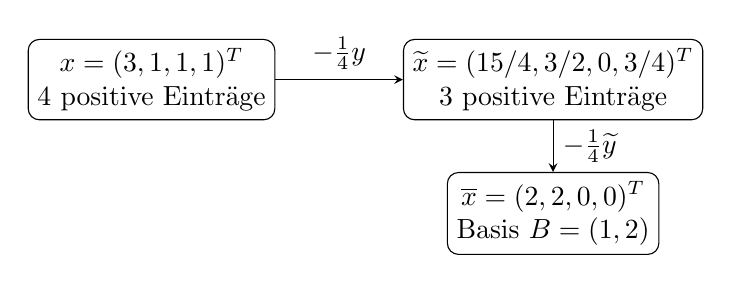
\begin{tikzpicture}[>=stealth]
\node[draw,rounded corners,align=center] (a) at (0,0) {$x=(3,1,1,1)^T$\\4 positive Einträge};
\node[draw,rounded corners,align=center] (b) at (5.1,0) {$\widetilde x=(15/4,3/2,0,3/4)^T$\\3 positive Einträge};
\node[draw,rounded corners,align=center] (c) at (5.1,-1.7) {$\overline x=(2,2,0,0)^T$\\Basis $B=(1,2)$};
\draw[->] (a)--node[above] {$-\frac14y$}(b);
\draw[->] (b)--node[right] {$-\frac14\widetilde y$}(c);
\end{tikzpicture}}

\aufgabe{4.3 (Programming)}
\angabe{For Example 2.2, maximize $-x_1+2x_2+6x_3$ subject to
\[
2x_1+3x_2+x_4=10,\qquad x_1+2x_3+x_5=8,\qquad
x_1+2x_2+x_3+x_6=6,\qquad x_1,\ldots,x_6\geq0.
\]
Determine $c,A,b$ and a basis $B$. Complete \texttt{initial\_simplex\_dictionary} from the supplied skeleton and test it on these data. Return the dimensions, $B,N$, $\overline b$, $\overline A$, $\overline z$, reduced costs, basic solution and feasibility. Submit the Python and PDF files as \texttt{LASTNAME\_sheet\_NUMBER.py} and \texttt{LASTNAME\_sheet\_NUMBER.pdf}.}
\teil{Data and initial basis}
\[
\boxed{c=\begin{pmatrix}-1\\2\\6\\0\\0\\0\end{pmatrix},\quad
A=\begin{pmatrix}2&3&0&1&0&0\\1&0&2&0&1&0\\1&2&1&0&0&1\end{pmatrix},\quad
b=\begin{pmatrix}10\\8\\6\end{pmatrix}.}
\]
Choose $B=(4,5,6)$ and $N=(1,2,3)$. The corresponding submatrices and costs are
\[
A_B=I_3,\quad A_N=\begin{pmatrix}2&3&0\\1&0&2\\1&2&1\end{pmatrix},\quad
c_B=\begin{pmatrix}0\\0\\0\end{pmatrix},\quad c_N=\begin{pmatrix}-1\\2\\6\end{pmatrix}.
\]
The columns of $I_3$ are independent, so $B$ is a basis.
\explain{Die letzten drei Spalten sind die Schlupfvariablen und bilden die Einheitsmatrix. Deshalb ist diese Basis für den Start praktisch. In der Mathematik zählen wir die Variablen ab eins. Python zählt ab null: Der Aufruf verwendet also \texttt{B=[3,4,5]}, nicht \texttt{[4,5,6]}. Die Reihenfolge bleibt wichtig, weil sie die Reihenfolge von $x_B$ und $\overline b$ festlegt.}
\teil{Dictionary quantities}
\begin{align*}
\overline b&=A_B^{-1}b&&\why{definition}\\
&=I_3b&&\why{inverse of the identity}\\
&=(10,8,6)^T&&\why{identity multiplication}\\
\overline A&=A_B^{-1}A_N&&\why{definition}\\
&=I_3A_N&&\why{inverse of the identity}\\
&=A_N&&\why{identity multiplication}\\
\overline z&=c_B^T\overline b&&\why{definition}\\
&=0\cdot10+0\cdot8+0\cdot6&&\why{substitute}\\
&=0+0+0&&\why{multiply}\\
&=0&&\why{add}\\
\overline c_N^T&=c_N^T-c_B^T\overline A&&\why{definition}\\
&=(-1,2,6)-(0,0,0)\overline A&&\why{substitute costs}\\
&=(-1,2,6)-(0,0,0)&&\why{zero row times matrix}\\
&=(-1,2,6)&&\why{subtract zero}
\end{align*}
\explain{Das Dictionary lautet $x_B=\overline b-\overline A x_N$. Die gespeicherte Matrix $\overline A$ trägt selbst kein zusätzliches Minuszeichen. Das Minus kommt erst in der Gleichung vor. Bei den reduzierten Kosten ziehen wir den Beitrag der Basisvariablen ab. Hier verschwindet er, weil deren Kosten alle null sind. Bei einer anderen Basis darf man diesen Term nicht weglassen.}
\begin{align*}
x_B&=\overline b-\overline A x_N&&\why{dictionary convention}\\
x_4&=10-2x_1-3x_2&&\why{first row}\\
x_5&=8-x_1-2x_3&&\why{second row}\\
x_6&=6-x_1-2x_2-x_3&&\why{third row}\\
z&=\overline z+\overline c_N^T x_N&&\why{objective dictionary}\\
&=0+(-1,2,6)(x_1,x_2,x_3)^T&&\why{substitute}\\
&=-x_1+2x_2+6x_3&&\why{row times column}
\end{align*}
For the basic solution set $x_N=(0,0,0)^T$:
\begin{align*}
x_4&=10-2\cdot0-3\cdot0&&\why{substitute}\\
&=10-0-0&&\why{multiply}\\
&=10&&\why{subtract zeros}\\
x_5&=8-0-2\cdot0&&\why{substitute}\\
&=8-0-0&&\why{multiply}\\
&=8&&\why{subtract zeros}\\
x_6&=6-0-2\cdot0-0&&\why{substitute}\\
&=6-0-0-0&&\why{multiply}\\
&=6&&\why{subtract zeros}
\end{align*}
All entries of $x_B$ are nonnegative. Check in the original system:
\begin{align*}
(Ax)_1&=2\cdot0+3\cdot0+10&&\why{substitute}\\
&=0+0+10&&\why{multiply}\\
&=10&&\why{add}\\
(Ax)_2&=0+2\cdot0+8&&\why{substitute}\\
&=0+0+8&&\why{multiply}\\
&=8&&\why{add}\\
(Ax)_3&=0+2\cdot0+0+6&&\why{substitute}\\
&=0+0+0+6&&\why{multiply}\\
&=6&&\why{add}\\
c^Tx&=-0+2\cdot0+6\cdot0&&\why{substitute}\\
&=0+0+0&&\why{multiply}\\
&=0&&\why{add}
\end{align*}
\[\boxed{(m,n)=(3,6),\quad x=(0,0,0,10,8,6)^T,\quad z=0,\quad\texttt{is\_feasible=True}.}\]
\explain{Nichtnegativität erlaubt auch null. Die Anfangslösung ist damit zulässig, aber wir behaupten nicht, dass sie optimal ist. Die Aufgabe verlangt nur, das Anfangs-Dictionary aufzubauen. Die positiven reduzierten Kosten zeigen hier sogar mögliche Verbesserungsrichtungen, solange die Nebenbedingungen sie zulassen.}
\teil{Python implementation and test}
The completed function is in \texttt{Bleier\_sheet\_4.py}. It retains the skeleton's keys and adds \texttt{x\_N} and the full vector \texttt{x}. It solves the systems $A_B\overline b=b$ and $A_B\overline A=A_N$ with \texttt{numpy.linalg.solve}; this computes the stated formulas without forming an inverse explicitly. Indices in the function are zero-based.

Run \texttt{python Bleier\_sheet\_4.py} for Example 2.2 and \texttt{python -m unittest -v test\_sheet4.py} for the tests. The example returns the quantities calculated above. The tests also reconstruct $Ax=b$ and the objective for a non-identity basis in a different column order, and check an infeasible basis, a degenerate feasible basis, invalid inputs and a singular basis.
\[\boxed{\overline b=(10,8,6)^T,\quad \overline A=A_N,\quad\overline z=0,\quad\overline c_N=(-1,2,6)^T.}\]
\explain{Im Code geben wir $c$ als eindimensionales Array ein. Das Produkt \texttt{c\_B @ A\_bar} entspricht dann der Zeile $c_B^T\overline A$. Die Formen der Arrays werden vor dem Rechnen geprüft. Eine singuläre Basis wird nicht als unzulässig markiert, sondern als Fehler gemeldet: Ohne invertierbare Basismatrix gibt es dieses Dictionary gar nicht. Für die Zulässigkeit übernimmt der Code genau den Vergleich aus dem Skelett, also \texttt{b\_bar >= 0} ohne Toleranz. Bei fast singulären Daten und Rundungsfehlern wäre eine gesonderte numerische Behandlung nötig; die ganzzahligen Beispieldaten bereiten hier kein Problem.}

\explain{
\section*{Classroom task 4.1 (learning supplement)}
\angabe{Given $x_3=-x_1+2x_2$, $x_4=4-2x_1+x_2$, $z=3x_1+x_2$ and $(x_1,x_2,x_3,x_4)=(0,0,0,4)$, let $x_1$ enter. Find the leaving variable and the basic feasible solution after the stated pivot $x_1=-x_3+2x_2$, $x_4=4+2x_3-3x_2$, $z=-3x_3+7x_2$.}
\begin{align*}
x_3&=-t&&\why{set $x_1=t$, keep $x_2=0$}\\
x_4&=4-2t&&\why{same substitution}\\
0-t&\geq0&&\why{nonnegativity of $x_3$}\\
0&\geq t&&\why{add $t$}\\
4-2t&\geq0&&\why{nonnegativity of $x_4$}\\
4&\geq2t&&\why{add $2t$}\\
2&\geq t&&\why{divide by 2}\\
t&=\min\{0/1,4/2\}&&\why{RHS divided by rate of decrease}\\
&=\min\{0,2\}&&\why{divide}\\
&=0&&\why{take minimum}
\end{align*}
$x_3$ ist bereits null und würde bei jedem positiven Schritt negativ. Deshalb verlässt $x_3$ die Basis schon bei Schrittlänge null. Das ist ein degenerierter Pivot. Die neue Basis unterscheidet sich, obwohl wir denselben Punkt behalten.
With new nonbasic variables $x_2=x_3=0$:
\begin{align*}
x_1&=-0+2\cdot0&&\why{substitute}\\
&=0+0&&\why{multiply}\\
&=0&&\why{add}\\
x_4&=4+2\cdot0-3\cdot0&&\why{substitute}\\
&=4+0-0&&\why{multiply}\\
&=4&&\why{remove zero terms}\\
z&=-3\cdot0+7\cdot0&&\why{substitute}\\
&=0+0&&\why{multiply}\\
&=0&&\why{add}
\end{align*}
Check in the old dictionary:
\begin{align*}
x_3&=-0+2\cdot0&&\why{substitute}\\
&=0+0&&\why{multiply}\\
&=0&&\why{add}\\
x_4&=4-2\cdot0+0&&\why{substitute}\\
&=4-0+0&&\why{multiply}\\
&=4&&\why{remove zeros}\\
z&=3\cdot0+0&&\why{substitute}\\
&=0+0&&\why{multiply}\\
&=0&&\why{add}
\end{align*}
\[\boxed{x_3\text{ leaves},\quad (x_1,x_2,x_3,x_4)=(0,0,0,4),\quad z=0.}\]
}
\end{document}
